% Figure
\begin{figure}[H]
	\centering
	\includegraphics[width=0.9\linewidth]{PH_FIGURE}
	\caption{PH CAPTION}
	\label{fig:PH_LABEL}
\end{figure}

% Figure with source
\begin{figure}[H]
	\centering
	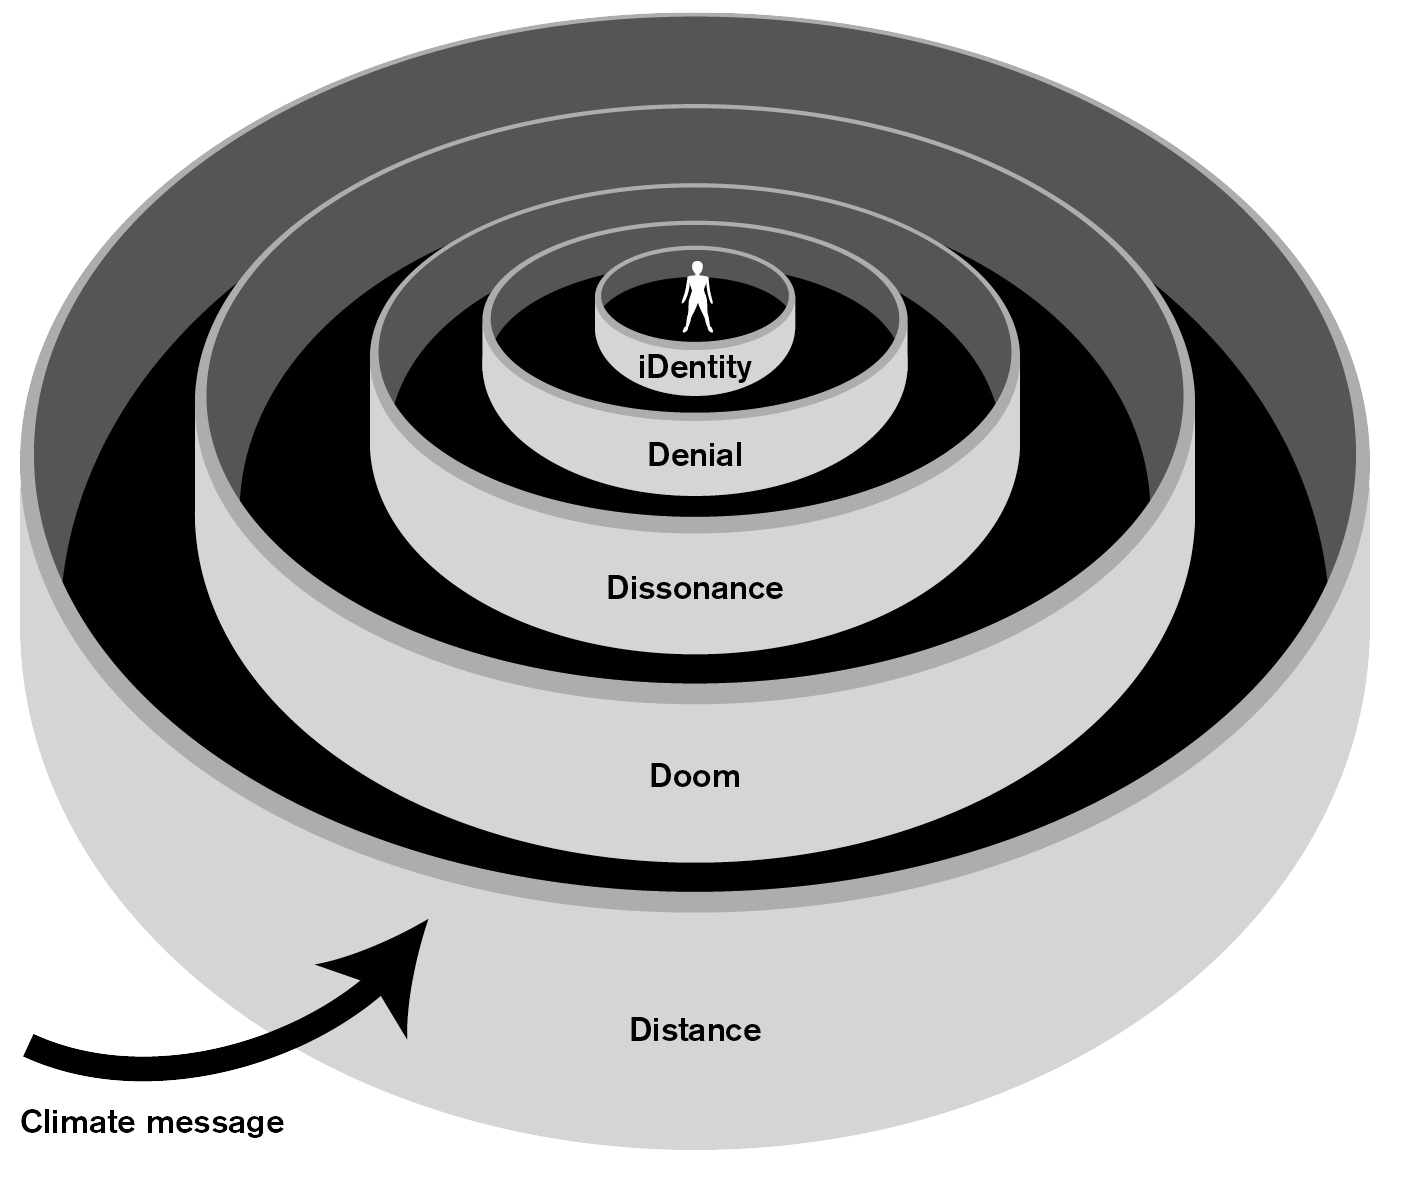
\includegraphics[width=0.9\linewidth]{figure/Analysis/5ds.png}
	\captionsource{The five psychological barriers blocking the climate message}{What we think about when we try not to think about global warming - Per Espen Stoknes\cite{storyAboutClimateChange} (2015)}
	\label{fig:5ds}
\end{figure}

% Items 'n lists
\begin{itemize}\label{stuff}
	\item[-] 
\end{itemize}

\begin{enumerate}
	\item [-]
\end{enumerate}

% Code related stuff
% Inline code highlight
The \mintinline{cpp}{Segment}

% Code snippet
\begin{listing}[H]
	\caption{PH_CAPTION}
	\label{listing:PH_LABEL}
	\begin{minted}[frame=lines,framesep=2mm,baselinestretch=1.1,fontsize=\footnotesize,linenos]{cpp}
PH_CODE
	\end{minted}
\end{listing}

% Citing stuff
@misc{miscTemplate,
	author = {Surname, name},
	title = {},
	url = {},
	note = {visited on xxxx-xx-xx}
	OPTmonth = {},
	OPTyear = {}
}

@book{bookTemplate,
	title = {},
	author = {Surname, Name},
	year = {},
	publisher = {}
}

@article{articleTemplate,
  author  = "Template, Author1 and Template Author2",
  title   = "Template title",
  journal = "Template Journal",
  year    = 2018,
}